%% Version 5.0, 2 January 2020
%
%%%%%%%%%%%%%%%%%%%%%%%%%%%%%%%%%%%%%%%%%%%%%%%%%%%%%%%%%%%%%%%%%%%%%%
% TemplateV5.tex --  LaTeX-based template for submissions to the 
% American Meteorological Society
%
%%%%%%%%%%%%%%%%%%%%%%%%%%%%%%%%%%%%%%%%%%%%%%%%%%%%%%%%%%%%%%%%%%%%%
% PREAMBLE
%%%%%%%%%%%%%%%%%%%%%%%%%%%%%%%%%%%%%%%%%%%%%%%%%%%%%%%%%%%%%%%%%%%%%

%% Start with one of the following:
% DOUBLE-SPACED VERSION FOR SUBMISSION TO THE AMS
\documentclass{ametsocV5}

% TWO-COLUMN JOURNAL PAGE LAYOUT---FOR AUTHOR USE ONLY
% \documentclass[twocol]{ametsocV5}


% Enter packages here. If too many math alphabets are used,
% remove unnecessary packages or define hmmax and bmmax as necessary.

%\newcommand{\hmmax}{0}
%\newcommand{\bmmax}{0}
\usepackage{amsmath,amsfonts,amssymb,bm}
\usepackage{mathptmx}%{times}
\usepackage{newtxtext}
\usepackage{newtxmath}


%%%%%%%%%%%%%%%%%%%%%%%%%%%%%%%%

%%% To be entered by author:

%% May use \\ to break lines in title:

\title{Hypernav Trajectory Prediction with PACIOOS Current Prediction and Ocean Parcels Software Package}

%%% Enter authors' names, as you see in this example:
%%% Use \correspondingauthor{} and \thanks{Current Affiliation:...}
%%% immediately following the appropriate author.
%%%
%%% Note that the \correspondingauthor{} command is NECESSARY.
%%% The \thanks{} commands are OPTIONAL.

    %\authors{Author One\correspondingauthor{Author name, email address}
% and Author Two\thanks{Current affiliation: American Meteorological Society, 
    % Boston, Massachusetts.}}

\authors{Paul Chamberlain\correspondingauthor{Paul Chamberlain, pchamber@ucsd.edu}}

%% Follow this form:
    % \affiliation{American Meteorological Society, 
    % Boston, Massachusetts}

%% If appropriate, add additional authors, different affiliations:
    %\extraauthor{Extra Author}
    %\extraaffil{Affiliation, City, State/Province, Country}

\extraauthor{Matt Mazloff}

\affiliation{Scripps Institution of Oceanography, 
La Jolla, California}
%\extraaffil{}

%% May repeat for a additional authors/affiliations:

%\extraauthor{}
%\extraaffil{}

%%%%%%%%%%%%%%%%%%%%%%%%%%%%%%%%%%%%%%%%%%%%%%%%%%%%%%%%%%%%%%%%%%%%%
% ABSTRACT
%
% Enter your abstract here
% Abstracts should not exceed 250 words in length!
%
 

\abstract{}

\begin{document}

%% Necessary!
\maketitle
\section{Introduction}
The Hypernav project proposes to seed the worlds oceans with Lagrangian hyper-spectral cameras based on the Argo platform \citep{roemmich2019future}, and offers an innovative means to validate the PACE satellite \citep{frouin2019atmospheric}. Floats built on the Argo platform are not Lagrangian drifters in the truest sense: argo floats are equipped with a small buoyancy engine which allows them to profile the water column while collecting ocean measurements, surface and broadcast those measurements, and then descend and drift at the so called "parking depth". Typical Core Argo floats drift at 1000 meters for 10 days before profiling. Because of operational limitations, Hypernav floats must drift shallower than 700 meters and surface daily. Determination of the ideal parking depth is the goal this study. Previous ocean color validation experiments have deployed instrumented moorings \citep{clark2003moby} to measure and transmit optical properties of the ocean. Instrumented moorings are typically expensive, difficult to maintain, and, because of their vastly greater size and weight, require complicated logistics to deploy globally; Lagrangian drifters on the other hand are typically less expensive than moorings and can be deployed by one or two people from the deck of almost any ship. Because of this scalability, proposals have been made to deploy a distributed network of Hypernav drifters globally. This global array will hypothetically validate ocean color measurements in many different climates and bioms as opposed to the one or two validation moorings that have been used to validate previous generations of ocean color satellites. This is not to say that Lagrangian drifters do not suffer from their own drawbacks. Drifters inherently move about with ocean currents; this is problematic for two reasons: firstly, instrumented drifters are fragile and cannot survive groundings. Care must be taken to navigate drifters at depths such that they avoid the ocean floor. Secondly, the regions of ideal satellite validations are relatively small. If Hypernav floats drift too far, their observations will not be useful for satellite validation. To address these challenges, we combine 2 technologies - the PACIOOS 4D prediction of currents in the Hawaiian Islands \citep{PacIOOS}, and the software package "Ocean Parcels" (Probably A Really Computationally Efficient Lagrangian Simulator)\citep{delandmeter2019parcels,Parcels} - to produce an almost real time prediction of float trajectories at 8 depth levels. Based on these predictions, deployed hypernav floats can be reprogrammed to drift at an ideal depth during incremental stages of its mission mission. The ideal park depth for this study is the depth at which the float has simultaneously the lowest probability of grounding and the highest probability of staying the required satellite calibration study area. The software package presented in this work is configured for the Hawaiian Islands, but this technique could be generally applied to any mission using the Argo platform. %need to include regional plot with float tracks

\section{Data}
The primary dataset used to create our predictions is the PACIOOS 4D ocean current prediction \citep{PacIOOS} and reanalysis \cite{partridge2019reanalysis}.
%include description of the way this model is created. 
For float trajectory prediction, data was downloaded from PACIOOS servers in a 2 degree box around the considered float position and 5 days in advance. 

Additionally, trajectories from Navis float 0042,xxx,xxx, and xxx %navis floats deployed during experiment
were used to validate the method. 


\section{Methods}
The method we imploy in these calculations is inherently quite simple and is 

\section{Results}

\section{Discussion}

\section{Conclusion}

%%%%%%%%%%%%%%%%%%%%%%%%%%%%%%%%%%%%%%%%%%%%%%%%%%%%%%%%%%%%%%%%%%%%%
% SIGNIFICANCE STATEMENT/CAPSULE SUMMARY
%%%%%%%%%%%%%%%%%%%%%%%%%%%%%%%%%%%%%%%%%%%%%%%%%%%%%%%%%%%%%%%%%%%%%
%
% If you are including an optional significance statement for a journal article or a required capsule summary for BAMS 
% (see www.ametsoc.org/ams/index.cfm/publications/authors/journal-and-bams-authors/formatting-and-manuscript-components for details), 
% please apply the necessary command as shown below:
%
% \statement
% Significance statement here.
%
% \capsule
% Capsule summary here.


%%%%%%%%%%%%%%%%%%%%%%%%%%%%%%%%%%%%%%%%%%%%%%%%%%%%%%%%%%%%%%%%%%%%%
% MAIN BODY OF PAPER
%%%%%%%%%%%%%%%%%%%%%%%%%%%%%%%%%%%%%%%%%%%%%%%%%%%%%%%%%%%%%%%%%%%%%
%

%% In all cases, if there is only one entry of this type within
%% the higher level heading, use the star form: 
%%
% \section{Section title}
% \subsection*{subsection}
% text...
% \section{Section title}

%vs

% \section{Section title}
% \subsection{subsection one}
% text...
% \subsection{subsection two}
% \section{Section title}

%%%
% \section{First primary heading}

% \subsection{First secondary heading}

% \subsubsection{First tertiary heading}

% \paragraph{First quaternary heading}

%%%%%%%%%%%%%%%%%%%%%%%%%%%%%%%%%%%%%%%%%%%%%%%%%%%%%%%%%%%%%%%%%%%%%
% ACKNOWLEDGMENTS
%%%%%%%%%%%%%%%%%%%%%%%%%%%%%%%%%%%%%%%%%%%%%%%%%%%%%%%%%%%%%%%%%%%%%
\acknowledgments
 Data provided by PacIOOS (www.pacioos.org), which is a part of the U.S. Integrated Ocean Observing System (IOOS), funded in part by National Oceanic and Atmospheric Administration (NOAA) Award \#NA16NOS0120024.


%%%%%%%%%%%%%%%%%%%%%%%%%%%%%%%%%%%%%%%%%%%%%%%%%%%%%%%%%%%%%%%%%%%%%
% DATA AVAILABILITY STATEMENT
%%%%%%%%%%%%%%%%%%%%%%%%%%%%%%%%%%%%%%%%%%%%%%%%%%%%%%%%%%%%%%%%%%%%%
% 
%
\datastatement
Output of model results and code are included as a supplement. Ocean Parcels software and documents can be found at https://oceanparcels.org/faq.html

%%%%%%%%%%%%%%%%%%%%%%%%%%%%%%%%%%%%%%%%%%%%%%%%%%%%%%%%%%%%%%%%%%%%%
% APPENDIXES
%%%%%%%%%%%%%%%%%%%%%%%%%%%%%%%%%%%%%%%%%%%%%%%%%%%%%%%%%%%%%%%%%%%%%
%
% Use \appendix if there is only one appendix.
%\appendix

% Use \appendix[A], \appendix[B], if you have multiple appendixes.
%\appendix[A]

%% Appendix title is necessary! For appendix title:
%\appendixtitle{}

%%% Appendix section numbering (note, skip \section and begin with \subsection)
% \subsection{First primary heading}

% \subsubsection{First secondary heading}

% \paragraph{First tertiary heading}

%% Important!
%\appendcaption{<appendix letter and number>}{<caption>} 
%must be used for figures and tables in appendixes, e.g.,
%
%\begin{figure}
%\noindent\includegraphics[width=19pc,angle=0]{figure01.pdf}\\
%\appendcaption{A1}{Caption here.}
%\end{figure}
%
% All appendix figures/tables should be placed in order AFTER the main figures/tables, i.e., tables, appendix tables, figures, appendix figures.
%
%%%%%%%%%%%%%%%%%%%%%%%%%%%%%%%%%%%%%%%%%%%%%%%%%%%%%%%%%%%%%%%%%%%%%
% REFERENCES
%%%%%%%%%%%%%%%%%%%%%%%%%%%%%%%%%%%%%%%%%%%%%%%%%%%%%%%%%%%%%%%%%%%%%
% Make your BibTeX bibliography by using these commands:
\bibliographystyle{ametsoc2014}
\bibliography{references}


%%%%%%%%%%%%%%%%%%%%%%%%%%%%%%%%%%%%%%%%%%%%%%%%%%%%%%%%%%%%%%%%%%%%%
% TABLES
%%%%%%%%%%%%%%%%%%%%%%%%%%%%%%%%%%%%%%%%%%%%%%%%%%%%%%%%%%%%%%%%%%%%%
%% Enter tables at the end of the document, before figures.
%%
%
%\begin{table}[t]
%\caption{This is a sample table caption and table layout.  Enter as many tables as
%  necessary at the end of your manuscript. Table from Lorenz (1963).}\label{t1}
%\begin{center}
%\begin{tabular}{ccccrrcrc}
%\hline\hline
%$N$ & $X$ & $Y$ & $Z$\\
%\hline
% 0000 & 0000 & 0010 & 0000 \\
% 0005 & 0004 & 0012 & 0000 \\
% 0010 & 0009 & 0020 & 0000 \\
% 0015 & 0016 & 0036 & 0002 \\
% 0020 & 0030 & 0066 & 0007 \\
% 0025 & 0054 & 0115 & 0024 \\
%\hline
%\end{tabular}
%\end{center}
%\end{table}

%%%%%%%%%%%%%%%%%%%%%%%%%%%%%%%%%%%%%%%%%%%%%%%%%%%%%%%%%%%%%%%%%%%%%
% FIGURES
%%%%%%%%%%%%%%%%%%%%%%%%%%%%%%%%%%%%%%%%%%%%%%%%%%%%%%%%%%%%%%%%%%%%%
%% Enter figures at the end of the document, after tables.
%%
%
% \begin{figure}[t]
%  \noindent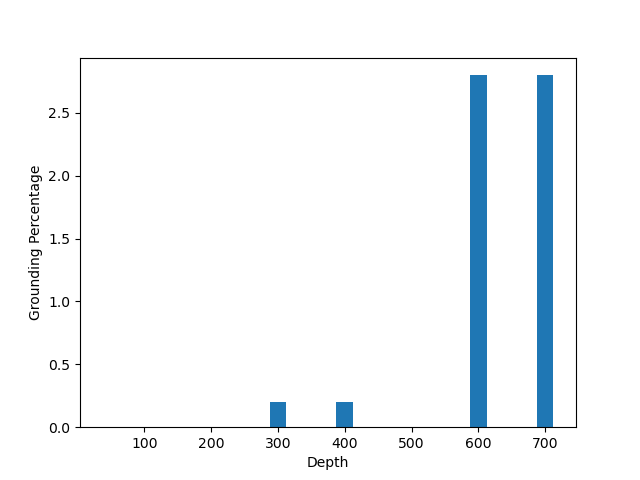
\includegraphics{../out/grounding_percentage.png}\\
%  \caption{Grounding Percentage for Float}
% \end{figure}

\end{document}